\documentclass[12pt]{article}

% Packages
\usepackage[margin=1.2in]{geometry}
\usepackage{amsmath,amssymb,amsthm}
\usepackage{microtype}
\usepackage{graphicx}
\usepackage{xcolor}
\definecolor{linkgreen}{RGB}{0,120,100}
\usepackage[colorlinks=true,linkcolor=linkgreen,citecolor=linkgreen,urlcolor=linkgreen]{hyperref}
\usepackage{natbib}
\usepackage{setspace}
\onehalfspacing

% Fix title font size (override \LARGE -> \Large so title fits in 2 lines)
\makeatletter
\def\@maketitle{%
  \newpage\null\vskip 1.5em%
  \begin{center}%
    {\Large\bfseries \@title \par}%
    \vskip 1em%
    {\normalsize\begin{tabular}[t]{c}\@author\end{tabular}\par}%
    \vskip 0.8em%
    {\normalsize \@date}%
  \end{center}\par\vskip 1.5em}
\makeatother

% Theorem environments
\theoremstyle{plain}
\newtheorem{proposition}{Proposition}
\newtheorem{lemma}{Lemma}
\newtheorem{corollary}{Corollary}
\theoremstyle{definition}
\newtheorem{assumption}{Assumption}
\newtheorem{definition}{Definition}
\theoremstyle{remark}
\newtheorem{remark}{Remark}

% Convenience macros
\newcommand{\pbar}{\bar{p}}
\newcommand{\lam}{\lambda}
\newcommand{\eps}{\varepsilon}
\newcommand{\EI}{E_{I}}
\newcommand{\PSB}{p^{SB}}
\newcommand{\Pcost}{p^{cost*}}
\newcommand{\1}{\mathbf{1}}
\DeclareMathOperator{\sgn}{sgn}

% -------------------------------------------------------------------
\title{Drug Procurement, Moral Hazard, and Originator Exit:\\
A Theoretical Framework}

\author{%
  \texttt{pAI-Econ-claude} (\texttt{theoretical-economics-claude-skill})\\[4pt]
  \small\url{https://github.com/maxwell2732/pAI-Econ-claude}\\[2pt]
  \small Claude Fable 5
}

\date{Draft: June 23, 2026. Revised: July 3, 2026.}
% -------------------------------------------------------------------

\begin{document}
\maketitle

\section{Introduction}

China's Volume-Based Procurement (VBP) policy centralizes pharmaceutical purchasing across public hospitals, replacing fragmented institution-level bargaining with competitive national auctions. Implemented starting in 2019, the policy has produced average price reductions of roughly 50 percent across successive procurement rounds, with some rounds achieving reductions exceeding 65 percent. The policy is explicitly motivated by cost containment: lower drug prices should reduce what the national medical insurance fund (BMI) spends on covered medicines.

This paper argues that the cost-containment logic is incomplete. When patients are insured, drug price reductions operate through two channels simultaneously: a \emph{savings channel} (each unit costs less) and an \emph{amplification channel} (lower out-of-pocket prices stimulate additional consumption through moral hazard). Whether insurance expenditure falls or rises depends on demand elasticity. More fundamentally, whether \emph{social welfare} rises depends on a third channel: the originator firm's participation decision. Originator pharmaceutical firms face fixed costs---research and development amortization, brand maintenance, regulatory compliance---that generic competitors do not. Below a threshold price, an originator cannot recover these fixed costs and exits the procurement market. This exit generates a discrete welfare discontinuity that may reverse the welfare gains from aggressive price reduction.

We develop a static partial-equilibrium model with four agents: an insurer (the VBP setter), an originator firm with positive fixed costs, a competitive generic industry, and $N$ insured patients. The model inherits the demand structure of \citet{Pauly1968} and \citet{Zeckhauser1970} but changes the policy instrument from the coinsurance rate to the regulated procurement price. Our main results are as follows.

\begin{enumerate}
\item \textbf{Expenditure tipping (Lemma~\ref{lem:expenditure}).} Insurance expenditure falls with the procurement price if and only if demand is inelastic at the prevailing out-of-pocket price ($\varepsilon < 1$). When demand is elastic, lower prices paradoxically raise total expenditure through moral hazard amplification.

\item \textbf{Participation threshold (Proposition~\ref{prop:threshold}).} A unique originator exit threshold $\bar{p}$ exists under standard regularity conditions. Over the VBP-relevant price range (below the originator's profit-maximizing price $p_O^{\max}$), the originator exits below $\bar{p}$ and participates above it.

\item \textbf{Insurance--exit complementarity (Proposition~\ref{prop:complement}).} More generous insurance ($\uparrow \lambda$) lowers the exit threshold: $\partial\bar{p}/\partial\lambda < 0$. Counterintuitively, generous public insurance enables more aggressive VBP without triggering originator withdrawal.

\item \textbf{Welfare kink at the exit threshold (Proposition~\ref{prop:kink}).} Social welfare has a discrete jump at $\bar{p}$ of magnitude $\Omega = NV_o - F - N(c_o - c_g)D((1-\lambda)\bar{p})$. When $\Omega > 0$, preserving originator variety improves welfare; when $\Omega < 0$, pushing the price below $\bar{p}$ (and triggering originator exit) is welfare-improving.

\item \textbf{Second-best VBP price (Proposition~\ref{prop:secondbest}).} The welfare-maximizing procurement price, holding insurance generosity fixed, sets patient out-of-pocket cost equal to supply marginal cost: $p^{SB} = c/(1-\lambda)$. This exceeds generic marginal cost $c_g$ whenever $\lambda > 0$.

\item \textbf{Insurer--planner wedge (Proposition~\ref{prop:wedge}).} A cost-minimizing insurer (the institutional objective of China's National Healthcare Security Administration) sets a price below the social optimum for inelastic essential drugs, amplifying moral hazard beyond what welfare maximization would tolerate.
\end{enumerate}

The paper is organized as follows. Section~\ref{sec:model} presents the model. Section~\ref{sec:results} states and proves the six results. Section~\ref{sec:discussion} develops the policy implications and discusses limitations. Section~\ref{sec:conclusion} concludes.

\section{Model}
\label{sec:model}

\subsection{Agents and Market Structure}

Consider a single drug category under a public health insurance system with centralized VBP. There are four types of agents.

\paragraph{Insurer / VBP setter (I).} A single government insurer announces a regulated procurement price $p \in [c_g, \infty)$ at which drugs will be purchased from participating firms and distributed to insured patients. The insurer is the Stackelberg leader.

\paragraph{Originator firm (O).} The originator has marginal cost $c_o > 0$ and fixed cost $F > 0$ (covering research and development amortization, brand maintenance, and regulatory compliance). The originator observes $p$ and decides whether to participate (supply at price $p$) or exit (earn zero). Its profit from participation is
\begin{equation}
\Pi_O(p) = (p - c_o) \cdot N \cdot D\!\left((1-\lambda)p\right) - F.
\label{eq:origprof}
\end{equation}

\paragraph{Generic industry (G).} A competitive fringe of generic firms with identical marginal cost $c_g \in (0, c_o)$ and zero fixed costs. Generics supply any demanded quantity at any price $p \geq c_g$, earning zero economic profit in equilibrium.

\paragraph{Patients (A).} There are $N > 0$ identical patients, each covered by insurance at coinsurance complement $\lambda \in (0,1)$: the patient pays $(1-\lambda)p$ per unit and the insurer pays $\lambda p$ per unit. Each patient has quasi-linear utility $u_i(q_i, x_i) = U(q_i) + x_i$ over drug consumption $q_i$ and a numeraire good $x_i$. Utility $U$ satisfies $U' > 0$, $U'' < 0$. The patient's optimal demand at out-of-pocket price $s = (1-\lambda)p$ is
\begin{equation}
q_i^* = D(s), \qquad \text{where } U'(D(s)) = s,
\label{eq:demand}
\end{equation}
so $D$ is the inverse of the marginal utility function $U'$.

\subsection{Timing}

\begin{enumerate}
\item \textbf{Insurer} announces $p \in [c_g, \infty)$, correctly anticipating downstream responses.
\item \textbf{Originator} observes $p$ and participates iff $\Pi_O(p) \geq 0$.
\item \textbf{Generic industry} supplies any demanded quantity at price $p$.
\item \textbf{Each patient} observes out-of-pocket price $(1-\lambda)p$ and demands $D((1-\lambda)p)$.
\item \textbf{Transfers:} insurer pays $\lambda p$ per unit; patients pay $(1-\lambda)p$ per unit; originator collects $(p - c_o)$ per unit if it participates, less fixed cost $F$.
\end{enumerate}

\subsection{Objectives and Welfare}

The insurer operates under two candidate objectives analyzed in parallel:

\paragraph{(a) Cost-minimizing insurer.} Minimize total insurance expenditure:
\begin{equation}
\EI(p) = \lambda \cdot p \cdot N \cdot D\!\left((1-\lambda)p\right).
\label{eq:expend}
\end{equation}

\paragraph{(b) Social welfare-maximizing planner.} Maximize:
\begin{equation}
W(p) = N\!\left[U\!\left(D(s)\right) - c(p)\,D(s)\right] - F\cdot\1\!\left[p \geq \pbar\right] + N V_o \cdot \1\!\left[p \geq \pbar\right],
\label{eq:welfare}
\end{equation}
where $s = (1-\lambda)p$, $c(p) = c_o$ if $p \geq \pbar$ (originator supplies) and $c(p) = c_g$ if $p < \pbar$ (generic only), $\1[\cdot]$ is the indicator function, $\pbar$ is the originator exit threshold defined below, and $V_o > 0$ is the per-patient welfare value of originator variety (availability, therapeutic differentiation).

The moral hazard deadweight loss at price $p$ is
\begin{equation}
\mathrm{DWL}(p) = N\!\left[U(D(c)) - c\,D(c)\right] - N\!\left[U(D(s)) - c\,D(s)\right] \geq 0,
\label{eq:dwl}
\end{equation}
since $D(c)$ maximizes the net social surplus $U(q) - cq$ and patients consume $D(s) > D(c)$ when $s = (1-\lambda)p < c$.

\subsection{Assumptions}

\begin{assumption}[Demand regularity]
\label{ass:demand}
$D:\mathbb{R}_+ \to \mathbb{R}_+$ is $C^2$, strictly decreasing ($D' < 0$), and weakly convex ($D'' \leq 0$). The demand elasticity $\varepsilon(s) \equiv -s\,D'(s)/D(s)$ is well-defined and positive for all $s > 0$.
\end{assumption}

\begin{assumption}[Fixed coinsurance]
\label{ass:lambda}
The coinsurance complement $\lambda \in (0,1)$ is an exogenous parameter (institutionally fixed by the BMI schedule); it is not a choice variable in the baseline model.
\end{assumption}

\begin{assumption}[Originator fixed cost]
\label{ass:fixedcost}
$F > 0$: the originator has strictly positive fixed costs.
\end{assumption}

\begin{assumption}[Market viability]
\label{ass:viable}
$\max_{p \geq c_g}(p - c_o)\cdot N \cdot D\!\left((1-\lambda)p\right) > F$: the originator's variable profit can cover its fixed cost at some price. Under Assumption~\ref{ass:demand} with linear demand $D(s) = a - bs$ ($a, b > 0$, $a > bc_o(1-\lambda)$), this requires $Nb(1-\lambda)\bigl(a/b(1-\lambda) - c_o\bigr)^2/4 > F$.
\end{assumption}

\begin{assumption}[Single-peaked originator profit]
\label{ass:singlepeaked}
$(p - c_o)\cdot D\!\left((1-\lambda)p\right)$ is single-peaked in $p$: strictly increasing on $(c_o, p_O^{\max})$ and strictly decreasing on $(p_O^{\max}, \infty)$, where $p_O^{\max}$ is the unconstrained profit-maximizing price. (Sufficient condition: $D$ is log-concave, which holds for linear and exponential demand.)
\end{assumption}

\section{Main Results}
\label{sec:results}

\subsection{Expenditure Tipping Effect}

When the insurer reduces the procurement price $p$, two forces operate on insurance expenditure $\EI$: the per-unit cost $\lambda p$ falls, but patient demand $D((1-\lambda)p)$ rises. The balance depends on demand elasticity.

\begin{lemma}[Expenditure tipping]
\label{lem:expenditure}
Under Assumption~\ref{ass:demand},
\begin{equation}
\frac{d\EI}{dp} = \lambda N D(s)\bigl[1 - \varepsilon(s)\bigr], \qquad s = (1-\lambda)p.
\label{eq:expendfoc}
\end{equation}
Hence $d\EI/dp > 0$ if $\varepsilon(s) < 1$ (inelastic demand: lower $p$ reduces expenditure) and $d\EI/dp < 0$ if $\varepsilon(s) > 1$ (elastic demand: lower $p$ raises expenditure). If $\varepsilon$ crosses unity, the \emph{tipping price} $\hat{p}$ defined by $\varepsilon((1-\lambda)\hat{p}) = 1$ is a local maximum of $\EI$.
\end{lemma}

\begin{proof}
Differentiate $\EI(p) = \lambda p N D((1-\lambda)p)$:
$$\frac{d\EI}{dp} = \lambda N\bigl[D(s) + p(1-\lambda)D'(s)\bigr].$$
Since $p(1-\lambda) = s$ and $s\,D'(s)/D(s) = -\varepsilon(s)$, factoring $\lambda N D(s)$ yields \eqref{eq:expendfoc}. The sign follows from $\lambda, N, D(s) > 0$.
\end{proof}

\begin{remark}
For essential drugs with inelastic demand ($\varepsilon < 1$ throughout), $\EI$ is strictly increasing in $p$, so the cost-minimizing insurer prefers the lowest feasible price $p = c_g$. The tipping price $\hat{p}$ is relevant only when demand transitions from inelastic to elastic over the range of VBP-plausible prices.
\end{remark}

\subsection{Originator Participation Threshold}

\begin{proposition}[Existence and uniqueness of exit threshold]
\label{prop:threshold}
Under Assumptions~\ref{ass:demand}--\ref{ass:singlepeaked}, there exists a unique $\pbar \in (c_o, p_O^{\max})$ such that, for all $p \in [c_g, p_O^{\max}]$, $\Pi_O(p) \geq 0$ if and only if $p \geq \pbar$. The threshold $\pbar$ is implicitly defined by
\begin{equation}
(\pbar - c_o)\cdot N \cdot D\!\left((1-\lambda)\pbar\right) = F.
\label{eq:threshold}
\end{equation}
Moreover, $\pbar$ is decreasing in $N$ (larger market) and increasing in $F$ (larger fixed cost).
\end{proposition}

\begin{proof}
$\Pi_O(c_o) = -F < 0$ by Assumption~\ref{ass:fixedcost}. By Assumption~\ref{ass:viable}, $\Pi_O(p_O^{\max}) > 0$. Since $\Pi_O$ is continuous (from Assumption~\ref{ass:demand}), the Intermediate Value Theorem gives at least one root $\pbar \in (c_o, p_O^{\max})$. Assumption~\ref{ass:singlepeaked} implies $\Pi_O$ is strictly increasing on $(c_o, p_O^{\max})$, so the root is unique on that interval, $\pbar$ is the lower zero-profit price, and the equivalence $\Pi_O(p) \geq 0 \Leftrightarrow p \geq \pbar$ holds for all $p \in [c_g, p_O^{\max}]$ (for $p \in [c_g, c_o]$, $\Pi_O(p) \leq -F < 0$). Monotonicity in $N$ and $F$ follows from implicit differentiation of \eqref{eq:threshold}.
\end{proof}

\begin{remark}[Upper participation boundary]
\label{rem:upperboundary}
The equivalence in Proposition~\ref{prop:threshold} does not extend to prices above $p_O^{\max}$: on the decreasing arm of variable profit, demand contraction eventually pushes $\Pi_O$ back below zero, so the participation set on $[c_g, \infty)$ is a bounded interval rather than a half-line. For example, with linear demand $D(s) = 10 - s$ and $(\lambda, c_o, F, N) = (0.7, 2, 0.5, 1)$, participation holds exactly on $[2.05,\, 33.28]$, while $p_O^{\max} = 17.67$. This upper boundary is irrelevant for VBP analysis---centralized procurement compresses prices \emph{downward} from the pre-VBP level, so the policy-relevant range lies well below $p_O^{\max}$---but the domain restriction in Proposition~\ref{prop:threshold} is necessary for the statement to be correct.
\end{remark}

\subsection{Insurance--Exit Complementarity}

The following result is the paper's secondary key finding and is counterintuitive: more generous insurance enables more aggressive VBP without triggering originator exit.

\begin{proposition}[Insurance--exit complementarity]
\label{prop:complement}
Under Assumptions~\ref{ass:demand}--\ref{ass:singlepeaked},
\begin{equation}
\frac{\partial\pbar}{\partial\lambda} < 0.
\label{eq:complement}
\end{equation}
A more generous insurance scheme (higher $\lambda$) lowers the originator exit threshold: at any given price, the originator earns higher profit because patients face a lower out-of-pocket price and demand more.
\end{proposition}

\begin{proof}
Define $G(p,\lambda) \equiv (p-c_o)\cdot N \cdot D((1-\lambda)p) - F$. At $(\pbar, \lambda)$, $G = 0$. Both partial derivatives of $G$ are needed.

\emph{Numerator of IFT expression:}
$$\frac{\partial G}{\partial\lambda}\bigg|_{\pbar} = -(\pbar - c_o)\cdot N \cdot \pbar \cdot D'((1-\lambda)\pbar) > 0,$$
since $\pbar > c_o$ and $D' < 0$.

\emph{Denominator of IFT expression:}
$$\frac{\partial G}{\partial p}\bigg|_{\pbar} = N\,D(s)\!\left[1 - \frac{\pbar - c_o}{\pbar}\,\varepsilon(s)\right], \quad s = (1-\lambda)\pbar.$$
At the lower threshold $\pbar$ (on the increasing arm of $\Pi_O$, by Assumption~\ref{ass:singlepeaked}), profit is increasing, so $\partial G/\partial p|_{\pbar} > 0$.

By the Implicit Function Theorem:
$$\frac{\partial\pbar}{\partial\lambda} = -\frac{\partial G/\partial\lambda}{\partial G/\partial p}\bigg|_{\pbar} = -\frac{(+)}{(+)} < 0. \qquad \square$$
\end{proof}

\begin{remark}
The conventional view holds that generous insurance and aggressive VBP are substitutes: if patients are well-insured, the policy rationale for driving prices lower is weaker. Proposition~\ref{prop:complement} shows the opposite on the originator participation margin: more generous insurance widens the set of VBP prices at which originators voluntarily participate. The implication for reform sequencing is direct: expanding BMI coverage before deepening VBP price cuts preserves originator participation over a larger range of prices.
\end{remark}

\subsection{Welfare Kink at the Exit Threshold}

The social welfare function inherits a discrete discontinuity at $\pbar$ from the originator's binary participation decision. This discontinuity is the central structural feature of the model.

\begin{proposition}[Welfare kink and optimal VBP strategy]
\label{prop:kink}
Under Assumptions~\ref{ass:demand}--\ref{ass:singlepeaked}, the welfare function $W(p)$ in \eqref{eq:welfare} has a discrete jump at $\pbar$. With tie-breaking in favour of originator participation at $p = \pbar$,
\begin{equation}
W(\pbar^+) - W(\pbar^-) = \Omega, \qquad \Omega \equiv N V_o - F - N(c_o - c_g)\,D\!\left((1-\lambda)\pbar\right).
\label{eq:omega}
\end{equation}
The optimal VBP strategy satisfies:
\begin{enumerate}
\item[(i)] If $\Omega > 0$ (variety-valuable): $p^* \geq \pbar$. Setting $p < \pbar$ triggers a welfare-reducing discrete loss.
\item[(ii)] If $\Omega < 0$ (variety-costly): $p^* < \pbar$ is consistent with higher welfare at the kink.
\item[(iii)] If $\Omega = 0$: $W$ is continuous at $\pbar$; welfare is unaffected by the participation margin.
\end{enumerate}
\end{proposition}

\begin{proof}
Taking one-sided limits of $W(p)$ as $p \to \pbar$ from above (originator in market, $c(p) = c_o$) and below (generic only, $c(p) = c_g$), and using continuity of $D((1-\lambda)\cdot)$ at $\pbar$:
\begin{align*}
W(\pbar^+) &= N\!\left[U(D(s_0)) - c_o\,D(s_0)\right] - F + NV_o, \\
W(\pbar^-) &= N\!\left[U(D(s_0)) - c_g\,D(s_0)\right],
\end{align*}
where $s_0 = (1-\lambda)\pbar$. The utility terms $N\,U(D(s_0))$ cancel. The difference is
$$W(\pbar^+) - W(\pbar^-) = N(c_g - c_o)D(s_0) - F + NV_o = NV_o - F - N(c_o-c_g)D(s_0) = \Omega.$$
The policy prescriptions (i)--(iii) follow immediately from the sign of $\Omega$.
\end{proof}

\begin{remark}
The net variety premium $\Omega$ in \eqref{eq:omega} includes three terms. The variety benefit $NV_o$ is the aggregate welfare gain from having the originator drug available. The fixed cost $-F$ is the social cost of keeping the originator operational. The supply-cost penalty $-N(c_o-c_g)D(\cdot)$ captures the allocative inefficiency of serving demand at the originator's higher marginal cost. For GQCE-certified generics---where bioequivalence certification establishes therapeutic equivalence with the originator---$V_o$ is small, and the supply-cost penalty may dominate, yielding $\Omega < 0$. Originator exit is then welfare-improving.
\end{remark}

\subsection{Second-Best VBP Price}

With $\lambda$ institutionally fixed (Assumption~\ref{ass:lambda}), the social planner chooses $p$ to maximize $W(p)$ on each smooth piece.

\begin{proposition}[Second-best procurement price]
\label{prop:secondbest}
Under Assumptions~\ref{ass:demand}--\ref{ass:lambda}, the interior second-best welfare-maximizing price on each piece of the domain is
\begin{equation}
p^{SB}_o = \frac{c_o}{1-\lambda} \quad \text{(originator piece, } p \geq \pbar\text{)}, \qquad p^{SB}_g = \frac{c_g}{1-\lambda} \quad \text{(generic piece, } p < \pbar\text{)}.
\label{eq:secondbest}
\end{equation}
At the second-best, patient out-of-pocket cost equals supply marginal cost, fully correcting the moral hazard distortion: $(1-\lambda)p^{SB} = c$.
\end{proposition}

\begin{proof}
On $[\pbar, \infty)$ with $c(p) = c_o$, differentiate $W(p)$:
$$\frac{dW}{dp} = N(1-\lambda)\,D'(s)\bigl[(1-\lambda)p - c_o\bigr] = N(1-\lambda)\,D'(s)\,\bigl[s - c_o\bigr].$$
Since $D'(s) < 0$ and $N(1-\lambda) > 0$, this expression equals zero at $s = c_o$, i.e., $(1-\lambda)p = c_o$. The second-order condition $d^2W/dp^2 = N(1-\lambda)^2 D'(c_o) < 0$ confirms a maximum. The argument for the generic piece is identical with $c_o$ replaced by $c_g$.
\end{proof}

\begin{remark}
The second-best price $p^{SB} = c/(1-\lambda)$ exceeds supply marginal cost $c$ by the factor $1/(1-\lambda) > 1$. For $\lambda = 0.7$ (a typical inpatient BMI reimbursement rate), $p^{SB} \approx 3.3c$. Since VBP competitive bidding in China typically drives prices toward generic manufacturing cost ($p_{\mathrm{VBP}} \approx c_g$), the actual VBP price systematically undershoots the social optimum: moral hazard is amplified beyond the second-best level.
\end{remark}

\subsection{Insurer--Planner Wedge}

The preceding remark motivates a formal comparison between the cost-minimizing insurer's optimum and the social planner's second-best.

\begin{proposition}[Insurer--planner wedge]
\label{prop:wedge}
Under Assumptions~\ref{ass:demand}--\ref{ass:lambda}, suppose demand is inelastic at all prices in $[c_g, \pbar]$: $\varepsilon((1-\lambda)p) < 1$ for all $p \in [c_g, \pbar]$. Then:
\begin{enumerate}
\item[(i)] The cost-minimizing insurer's optimal price is the corner solution $\Pcost = c_g$.
\item[(ii)] $\Pcost < p^{SB}_g = c_g/(1-\lambda)$, with wedge $p^{SB}_g - \Pcost = c_g\lambda/(1-\lambda) > 0$.
\item[(iii)] At $\Pcost$, the deadweight loss $\mathrm{DWL}(\Pcost) > 0$; at $p^{SB}_g$, $\mathrm{DWL}(p^{SB}_g) = 0$.
\end{enumerate}
\end{proposition}

\begin{proof}
(i) By Lemma~\ref{lem:expenditure}, $d\EI/dp > 0$ when $\varepsilon < 1$. Hence $\EI$ is strictly increasing on $[c_g, \pbar]$, and the unique minimizer is the left endpoint $p = c_g$.

(ii) $p^{SB}_g = c_g/(1-\lambda)$. Since $\lambda > 0$, $(1-\lambda) < 1$, so $c_g/(1-\lambda) > c_g = \Pcost$. The wedge equals $c_g\lambda/(1-\lambda)$.

(iii) At $p^{SB}_g$, $(1-\lambda)p^{SB}_g = c_g$, so patients face marginal cost and $\mathrm{DWL} = 0$ by definition \eqref{eq:dwl}. At $\Pcost = c_g$, $(1-\lambda)c_g < c_g$, so patients consume $D((1-\lambda)c_g) > D(c_g)$, yielding $\mathrm{DWL} > 0$.
\end{proof}

\begin{remark}
The insurer, by minimizing its own expenditure outlay, drives the procurement price to the generic marginal cost floor. This achieves the insurer's narrow mandate but imposes a social cost: patient out-of-pocket price $(1-\lambda)c_g$ falls below marginal cost, inducing over-consumption. The social planner would set a higher price $p^{SB}_g = c_g/(1-\lambda)$ to eliminate this distortion---paying more per unit but inducing less over-consumption. The insurer's ``cost containment'' policy is counterproductive from a social welfare perspective: it reduces per-unit costs while amplifying demand beyond socially efficient levels. The inelasticity hypothesis is essential to the direction of the wedge: if demand is elastic ($\varepsilon > 1$) throughout the feasible range, $\EI$ is \emph{decreasing} in $p$ and the cost-minimizing insurer instead prefers the highest feasible price, placing $\Pcost$ \emph{above} the second-best price. The wedge sign asserted here is therefore a statement about essential drugs with inelastic demand, not a general property of the model.
\end{remark}

\subsection{Numerical Illustration}
\label{sec:numerical}

Figures~\ref{fig:welfarekink} and~\ref{fig:regimemap} illustrate the paper's central objects computationally. Neither figure is a proof; both are fully reproducible from the simulation scripts archived with the project (\texttt{outputs/numerical\_code/}, fixed seed, one-command rerun), and the parameter values are illustrative rather than calibrated.

Figure~\ref{fig:welfarekink} plots $W(p)$ for the linear-demand specification. It displays the two results that organize Section~4: the discrete welfare drop at the participation boundary $\pbar$ (Proposition~\ref{prop:kink}, here with $\Omega < 0$), and the interior second-best critical point at $p = c_o/(1-\lambda)$ on the originator branch (Proposition~\ref{prop:secondbest}). At these parameter values the global optimum lies at the kink, approached from the generic side---an honest reminder that the interior originator-branch optimum characterized in Proposition~\ref{prop:secondbest} is a local optimum whose global status depends on the sign of $\Omega$.

Figure~\ref{fig:regimemap} sweeps demand curvature $\varepsilon_0$ (CES family $D(s) = s^{-\varepsilon_0}$) against the originator fixed cost $F$ and classifies the location of $\arg\max_p W(p)$. The map shows that all three regimes discussed in the text arise on open parameter regions: for high $F$ the optimum is interior on the generic branch (originator variety not worth preserving); for low $F$ and high curvature it is interior on the originator branch; and on a broad intermediate band the optimum sits exactly at the kink $\pbar$, where the participation constraint binds.

\begin{figure}[t]
\centering
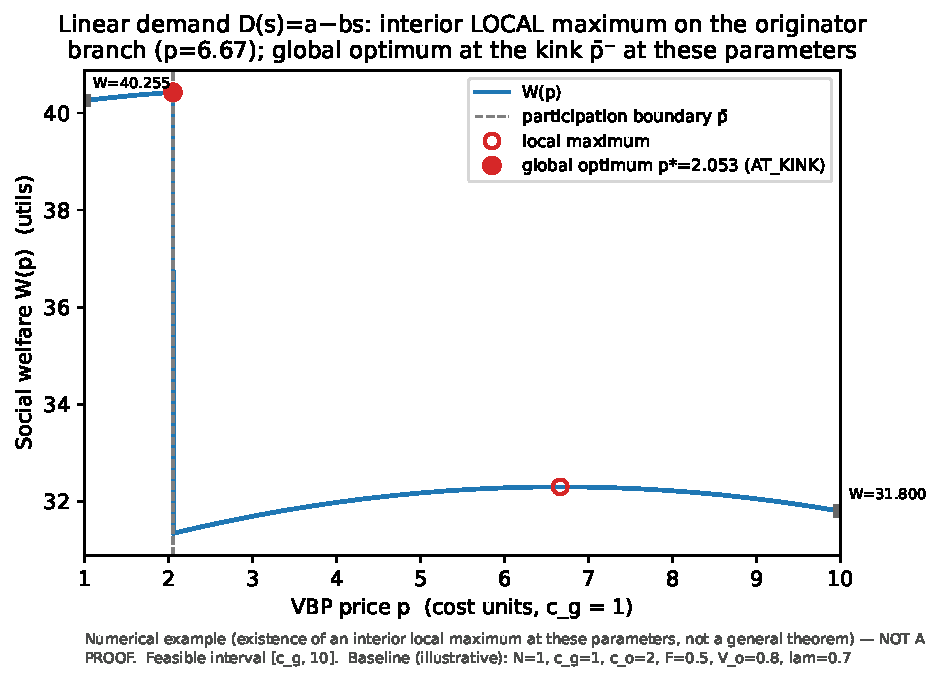
\includegraphics[width=0.82\textwidth]{numerical_figures/welfare_linear_interior.pdf}
\caption{\textbf{Welfare kink and interior local optimum (numerical example --- not a proof).} Social welfare $W(p)$ under linear demand $D(s) = 10 - s$ with illustrative parameters $(N, c_g, c_o, F, V_o, \lambda) = (1, 1, 2, 0.5, 0.8, 0.7)$. The dashed line marks the participation boundary $\pbar = 2.05$; open markers are interior local maxima; the filled marker is the global optimum. Reproducible from \texttt{numerical\_code/generate\_figures.py}.}
\label{fig:welfarekink}
\end{figure}

\begin{figure}[t]
\centering
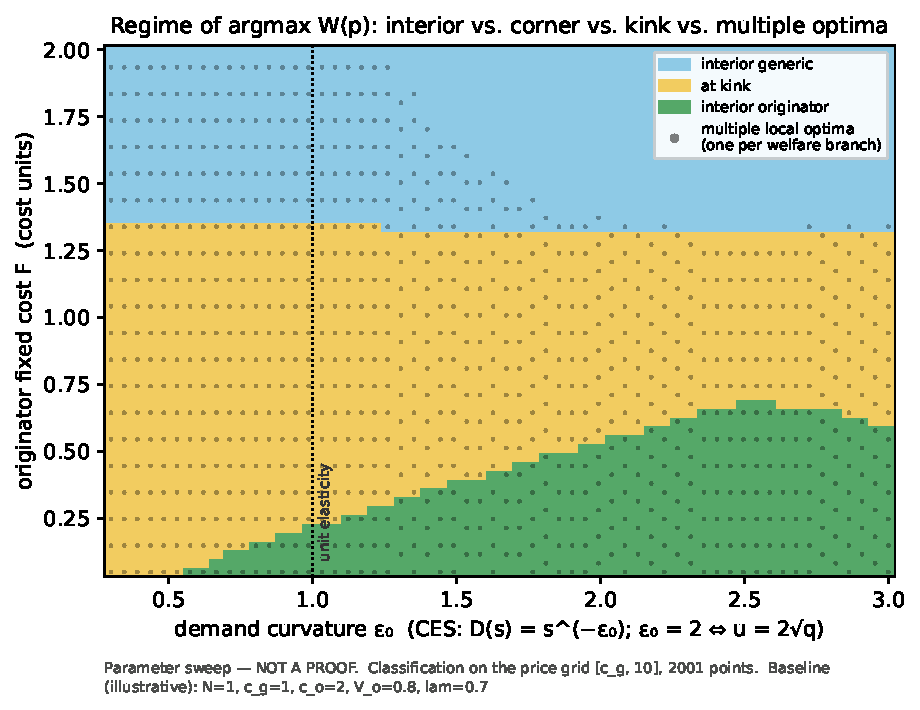
\includegraphics[width=0.85\textwidth]{numerical_figures/regime_map.pdf}
\caption{\textbf{Regime map of the second-best price (parameter sweep --- not a proof).} Location of $\arg\max_p W(p)$ over demand curvature $\varepsilon_0 \in [0.3, 3]$ and originator fixed cost $F \in [0.05, 2]$ (CES demand; other parameters at the illustrative baseline; price grid $[c_g, 10]$ with 2{,}001 points). Dots mark parameter combinations with multiple local optima (one per welfare branch). Reproducible from \texttt{numerical\_code/parameter\_sweep.py} and \texttt{generate\_figures.py}.}
\label{fig:regimemap}
\end{figure}

\section{Discussion}
\label{sec:discussion}

\subsection{Policy Prescriptions}

The six results yield specific policy prescriptions for VBP design:

\paragraph{Demand elasticity testing before price-setting.} Lemma~\ref{lem:expenditure} suggests that policymakers estimate demand elasticities before fixing VBP prices. If the OOP demand elasticity exceeds unity at the intended VBP price, a further price reduction raises insurance expenditure---the opposite of the policy objective. The tipping price $\hat{p}$ (where $\varepsilon = 1$) provides an empirical threshold.

\paragraph{Sequence insurance expansion before price cuts.} Proposition~\ref{prop:complement} ($\partial\pbar/\partial\lambda < 0$) implies a specific reform order: expand BMI coverage generosity (raise $\lambda$) before deepening VBP price reductions (lower $p$ toward $c_g$). Under more generous insurance, the same level of VBP aggressiveness yields lower originator exit risk. China's ongoing expansion of outpatient BMI coverage---extending the higher inpatient reimbursement rate to more drug categories---is consistent with this sequencing.

\paragraph{Calibrate $\Omega$ by drug type.} The welfare kink condition $\Omega > 0$ (Proposition~\ref{prop:kink}) depends on whether originator variety value $V_o$ exceeds the sum of fixed cost $F$ and supply-cost penalty $N(c_o - c_g)D(\cdot)$. For GQCE-certified generics with established bioequivalence, $V_o$ is low and $\Omega < 0$: aggressive VBP (pushing $p < \pbar$) is welfare-improving. For complex biologics, reference-listed drugs without generic competitors, or drugs where patient--drug matching matters clinically, $V_o$ is larger and $\Omega$ may be positive: a minimum price floor at $\pbar$ is welfare-warranted.

\paragraph{Reform the insurer's objective function.} Proposition~\ref{prop:wedge} reveals a structural misalignment between the NHSA's cost-minimization mandate and social welfare. The wedge $c_g\lambda/(1-\lambda)$ is not small: at $\lambda = 0.7$ and $c_g = 10$ yuan/unit, the social optimum is at 33 yuan/unit while the cost-minimizing insurer drives to 10 yuan/unit. Introducing a welfare-augmented mandate---requiring the NHSA to weigh moral hazard costs and variety preservation alongside expenditure---would close this gap.

\subsection{Counterintuitive Findings and Caveats}

Three findings deserve emphasis because they contradict common policy intuitions.

First, generous insurance does not make the case for VBP weaker (as a naive substitutability argument would suggest). It makes aggressive VBP \emph{more} survivable for originators. However, simultaneous with this complementarity, more generous insurance reduces the net variety premium $\Omega$ (because demand at the threshold rises, increasing the supply-cost penalty). The two effects operate in opposite directions: insurance generosity helps with the \emph{participation} margin but hurts on the \emph{variety value} margin.

Second, social welfare may be higher with originator exit than without, even when $V_o > 0$. The supply-cost penalty $N(c_o - c_g)D(\cdot)$ can dominate, making generic-only supply the welfare-superior outcome. This is the model's formal rationale for the GQCE certification program: by certifying bioequivalence, policymakers reduce $V_o$ for affected drugs, making originator exit welfare-neutral or welfare-improving.

Third, the cost-minimizing insurer drives prices too \emph{low} for welfare, not too high. A common critique of government health insurance is that it may set prices above cost (to protect incumbent firms). This model shows the opposite for essential drugs under competitive VBP: expenditure minimization drives prices to the floor, over-stimulating demand through moral hazard.

\subsection{Scope Limitations}

This paper abstracts from several important channels.

\paragraph{Dynamic R\&D incentives.} The model is static. Originator exit from VBP markets reduces expected returns from R\&D, potentially reducing future drug innovation---a long-run welfare cost not captured in the static model.

\paragraph{Physician moral hazard.} Physician prescribing incentives (historically significant in China's drug market before the 2015--2018 anti-corruption reforms) are excluded. Adding a physician layer would introduce a second moral hazard channel, strengthening the case for VBP price reduction but complicating the welfare calculation.

\paragraph{Heterogeneous insurance coverage.} Patients are assumed identical with uniform $\lambda$. China's BMI system features wide variation in $\lambda$ across facility types and insurance pools ($\lambda \approx 0.3$--$0.8$). Heterogeneous coverage would change the demand aggregation and the access-equity implications, but the qualitative comparative statics are preserved.

\paragraph{General equilibrium.} Interactions between VBP and pharmaceutical R\&D markets, hospital budget constraints, and foreign direct investment in China's pharmaceutical sector are excluded by the partial equilibrium assumption.

\section{Conclusion}
\label{sec:conclusion}

This paper develops a health insurance moral hazard model tailored to China's Volume-Based Procurement policy. The central finding is that the social welfare function has a discrete discontinuity at the originator exit threshold $\pbar$, with a welfare jump of magnitude $\Omega = NV_o - F - N(c_o-c_g)D((1-\lambda)\pbar)$. Whether VBP should push prices below $\pbar$ depends on the sign of $\Omega$---a criterion that depends on drug-specific parameters (variety value, fixed cost differential, demand at the threshold) and can in principle be estimated from data.

The model's secondary result---$\partial\pbar/\partial\lambda < 0$, the complementarity between insurance generosity and VBP aggressiveness---has implications for reform sequencing: expanding BMI coverage before deepening price cuts preserves originator participation over a larger policy space. The insurer--planner wedge (Proposition~\ref{prop:wedge}) suggests a structural conflict between the NHSA's cost-minimization mandate and social welfare maximization that cannot be resolved by adjusting the procurement price alone; the insurer's objective function itself may need to be reformed.

Together, the six results provide a framework for evaluating VBP design choices that integrates moral hazard, firm participation, and welfare analysis in a single tractable model.

% References
\begin{thebibliography}{99}

\bibitem[Arrow(1963)]{Arrow1963}
Arrow, K.J. (1963).
\newblock Uncertainty and the welfare economics of medical care.
\newblock \emph{American Economic Review}, 53(5):941--973.

\bibitem[Laffont and Tirole(1993)]{LT1993}
Laffont, J.-J. and Tirole, J. (1993).
\newblock \emph{A Theory of Incentives in Procurement and Regulation}.
\newblock MIT Press, Cambridge, MA.

\bibitem[Manning et al.(1987)]{Manning1987}
Manning, W.G., Newhouse, J.P., Duan, N., Keeler, E.B., Leibowitz, A., and Marquis, M.S. (1987).
\newblock Health insurance and the demand for medical care: Evidence from a randomized experiment.
\newblock \emph{American Economic Review}, 77(3):251--277.

\bibitem[Newhouse(1993)]{Newhouse1993}
Newhouse, J.P. (1993).
\newblock \emph{Free for All? Lessons from the RAND Health Insurance Experiment}.
\newblock Harvard University Press, Cambridge, MA.

\bibitem[Pauly(1968)]{Pauly1968}
Pauly, M.V. (1968).
\newblock The economics of moral hazard: Comment.
\newblock \emph{American Economic Review}, 58(3):531--537.

\bibitem[Shleifer(1985)]{Shleifer1985}
Shleifer, A. (1985).
\newblock A theory of yardstick competition.
\newblock \emph{RAND Journal of Economics}, 16(3):319--327.

\bibitem[Zeckhauser(1970)]{Zeckhauser1970}
Zeckhauser, R. (1970).
\newblock Medical insurance: A case study of the tradeoffs between risk spreading and appropriate incentives.
\newblock \emph{Journal of Economic Theory}, 2(1):10--26.

\end{thebibliography}

\end{document}
